\begin{frame}
    \frametitle{Factoring, motivation}
\note{Filename: ccsd\_factoring01.tex}

\small
\begin{block}{Diagram (2.12)}
    \begin{equation*}
        \parbox{40mm}{
\includegraphics[scale=0.5]{graphics/ccsd_hbar_13_12}}
        = \frac{1}{4}  \bra{mn}\ket{ef} t_{ij}^{ef} t_{mn}^{ab}
    \end{equation*}
\end{block}
\begin{block}{Diagram (2.26)}
    \begin{equation*}
        \parbox{40mm}{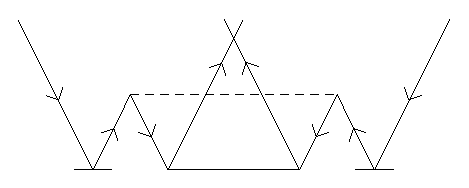
\includegraphics[scale=0.5]{graphics/ccsd_hbar_13_26}}
        = \frac{1}{4} P(ij) \bra{mn}\ket{ef} t_i^e t_{mn}^{ab} t_j^f
    \end{equation*}
\end{block}
\begin{block}{Diagram (2.31)}
    \begin{equation*}
        \parbox{40mm}{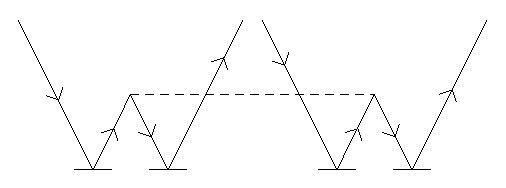
\includegraphics[scale=0.5]{graphics/ccsd_hbar_13_31}}
        = \frac{1}{4} P(ij) P(ab) \bra{mn}\ket{ef} t_i^e t_m^a t_j^f t_n^b
    \end{equation*}
\end{block}
\end{frame}

